\chapter{Iteration Plan 2 (FYP 1 Final)}
\label{ch:iter2}
This chapter outlines the second iteration plan for our project, providing guidance on module development and addressing students' discussion on the second stage of implementation method.

\section{FYP 1 Final:}
\begin{itemize}
    \item FYP 1 Final Presentation: \begin{itemize}
    \item Environment setup in Unity3D and Blender 
    \item Designed basic environment of Hospital
    \end{itemize}
\end{itemize}

\section{Designed basic environment of Hospital:}
	\begin{itemize}
	\item Reception Area
	\item Waiting Rooms
	\item Patient Rooms
	\item Training Facilities
\end{itemize}	
	
\subsection{Hospital Entrance:}
The hospital entrance serves as the main entry point to the virtual hospital
	\begin{figure}[h]
		\centering
		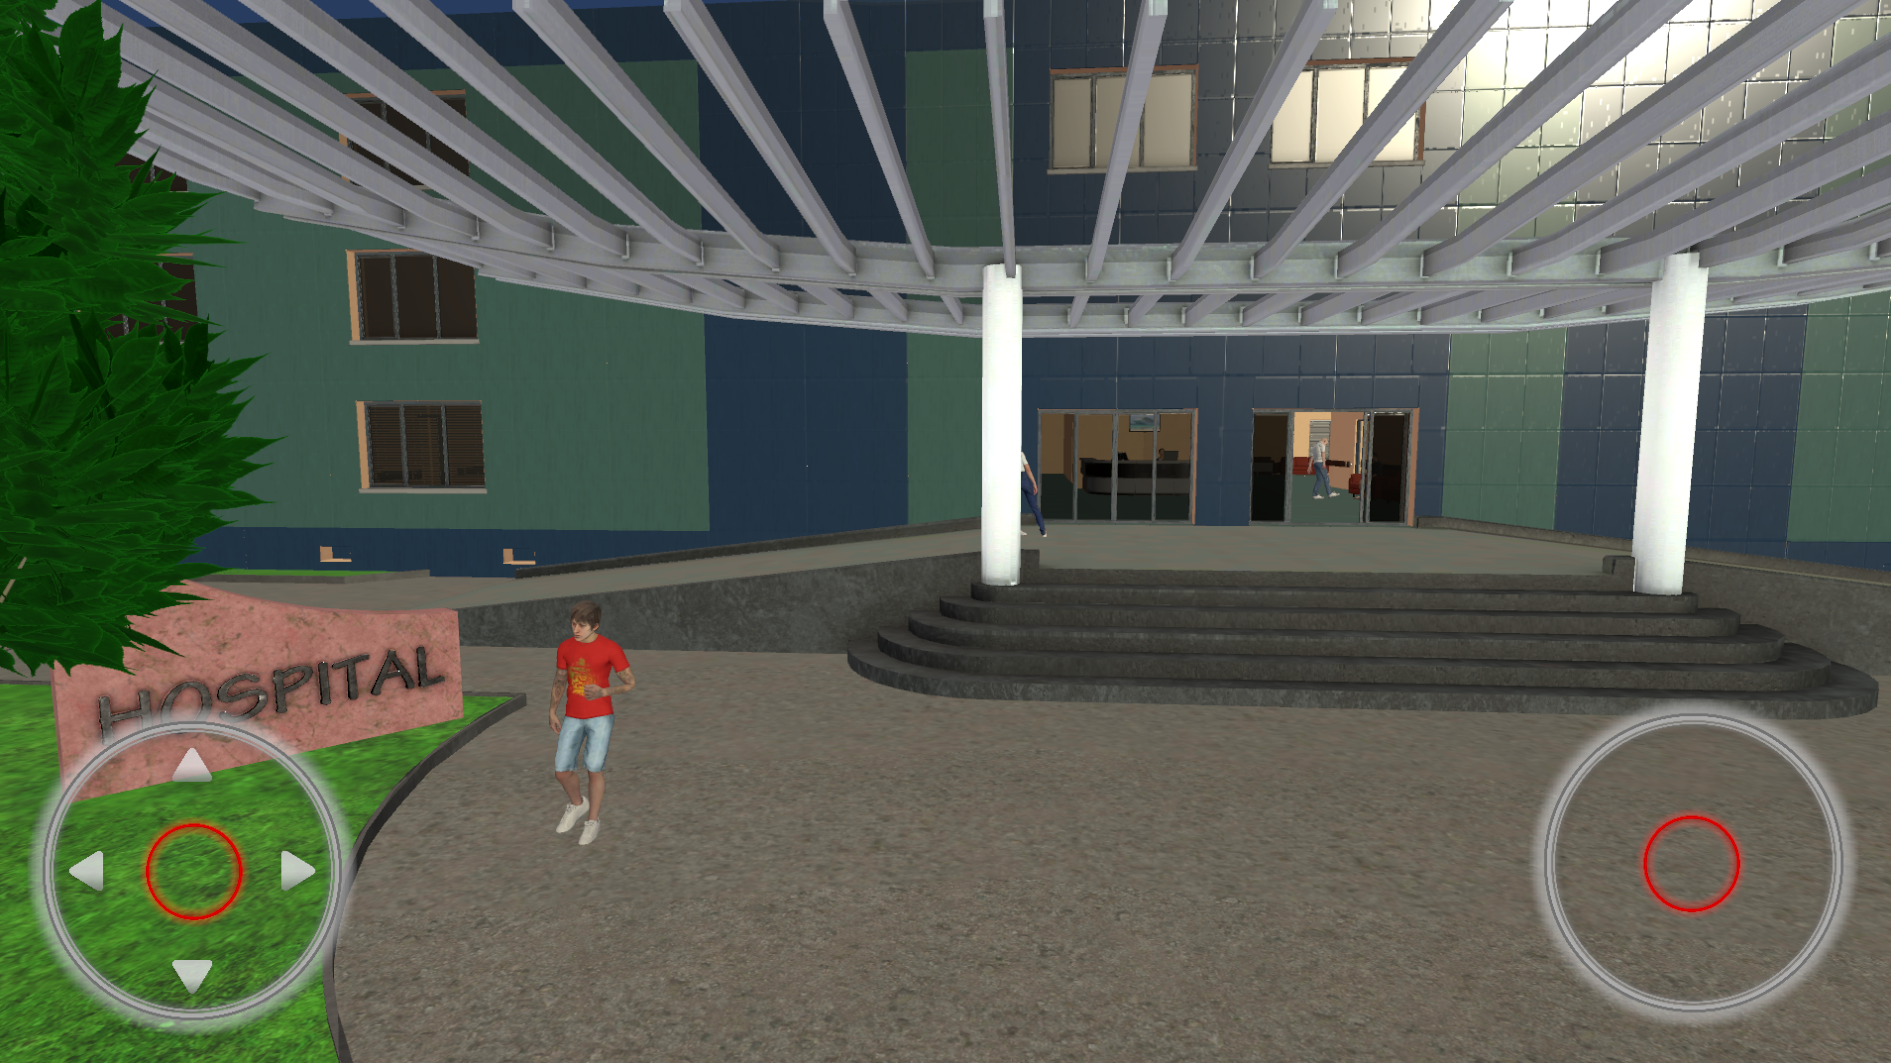
\includegraphics[width=0.5\textwidth, height=0.3\textheight]{Images/Hospital Enterance.png}
		\caption{Hospital Enterance}
		\label{fig:system-diagram}
	\end{figure}
\newline

\subsection{Reception Area:}
The reception area is the primary entrance to the virtual hospital, where patients and visitors can check-in and provide necessary information.
\begin{figure}[h]
	\centering
	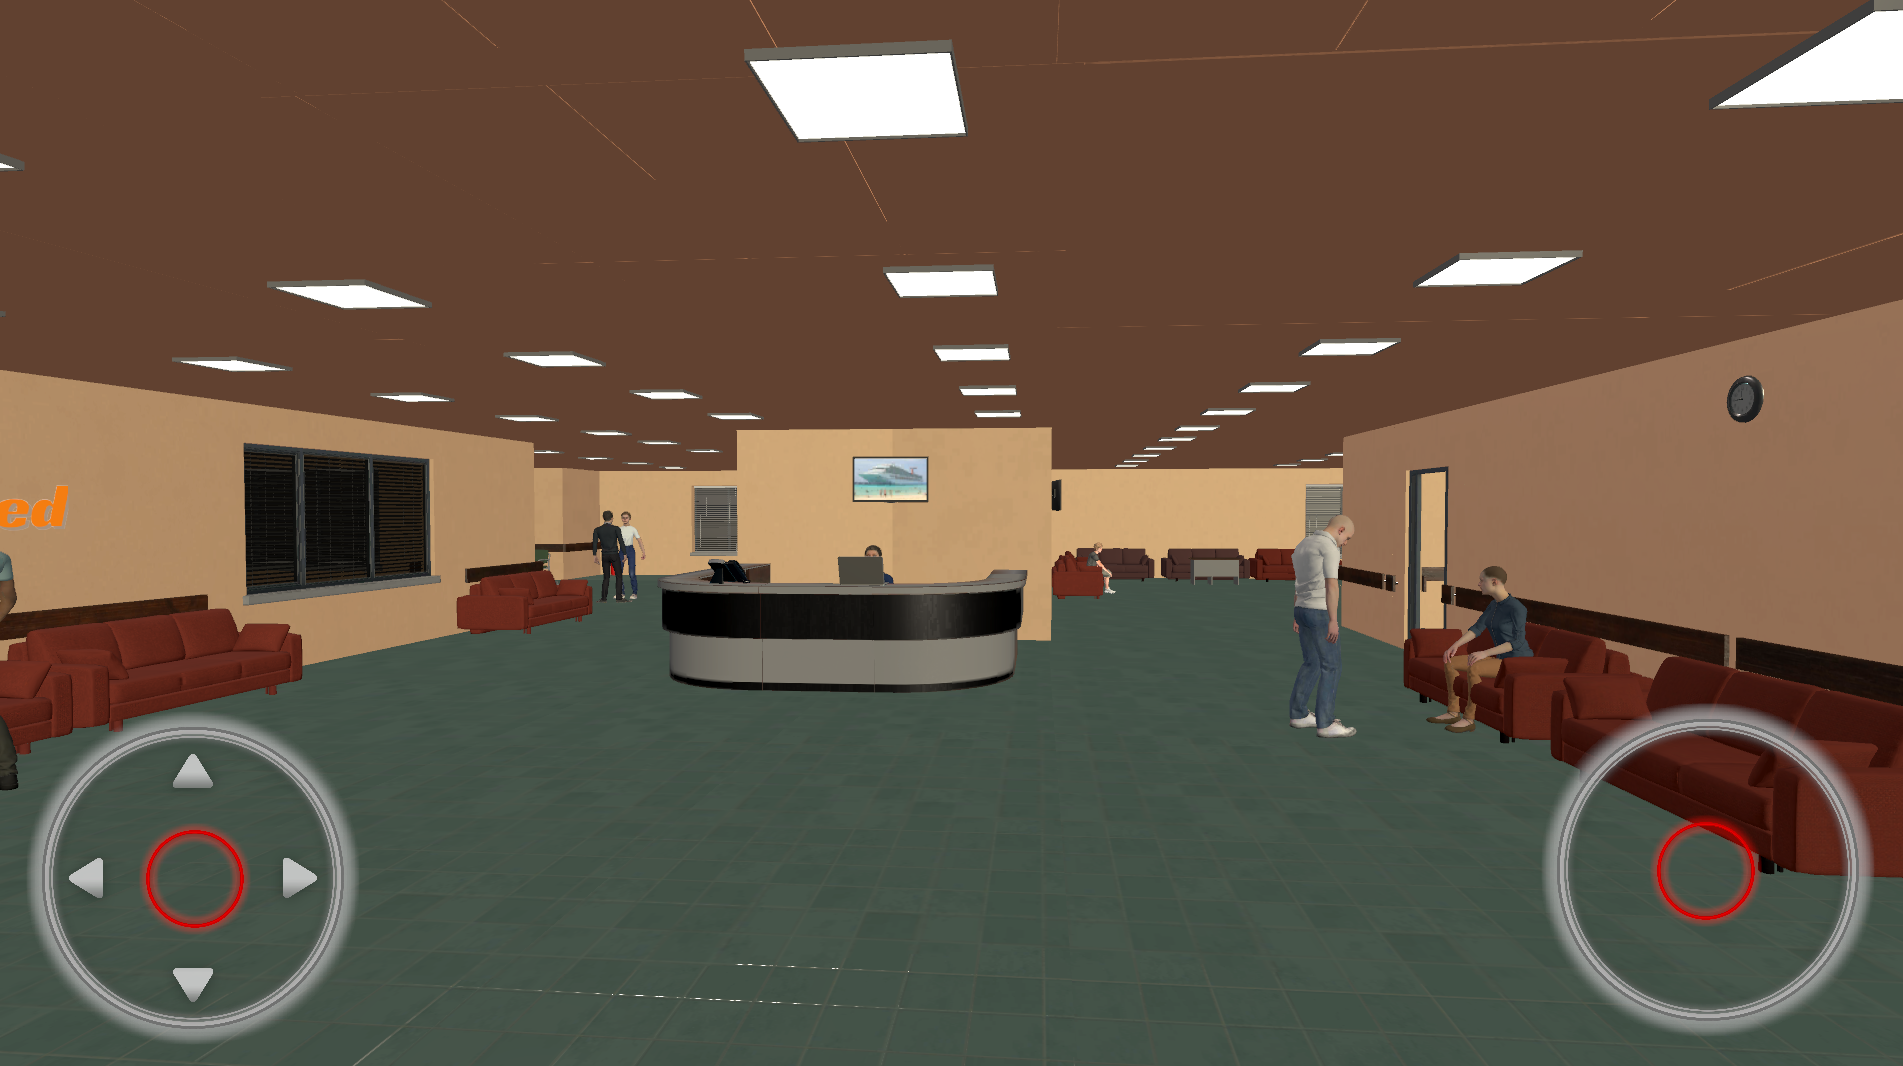
\includegraphics[width=0.5\textwidth, height=0.3\textheight]{Images/Reception Area.png}
	\caption{Reception Area}
	\label{fig:system-diagram}
\end{figure}
\newline

\subsection{Waiting Area:}	
Waiting area is designed to provide comfortable seating arrangements for patients and their companions while they wait for appointments or procedures.
\begin{figure}[h]
		\centering
		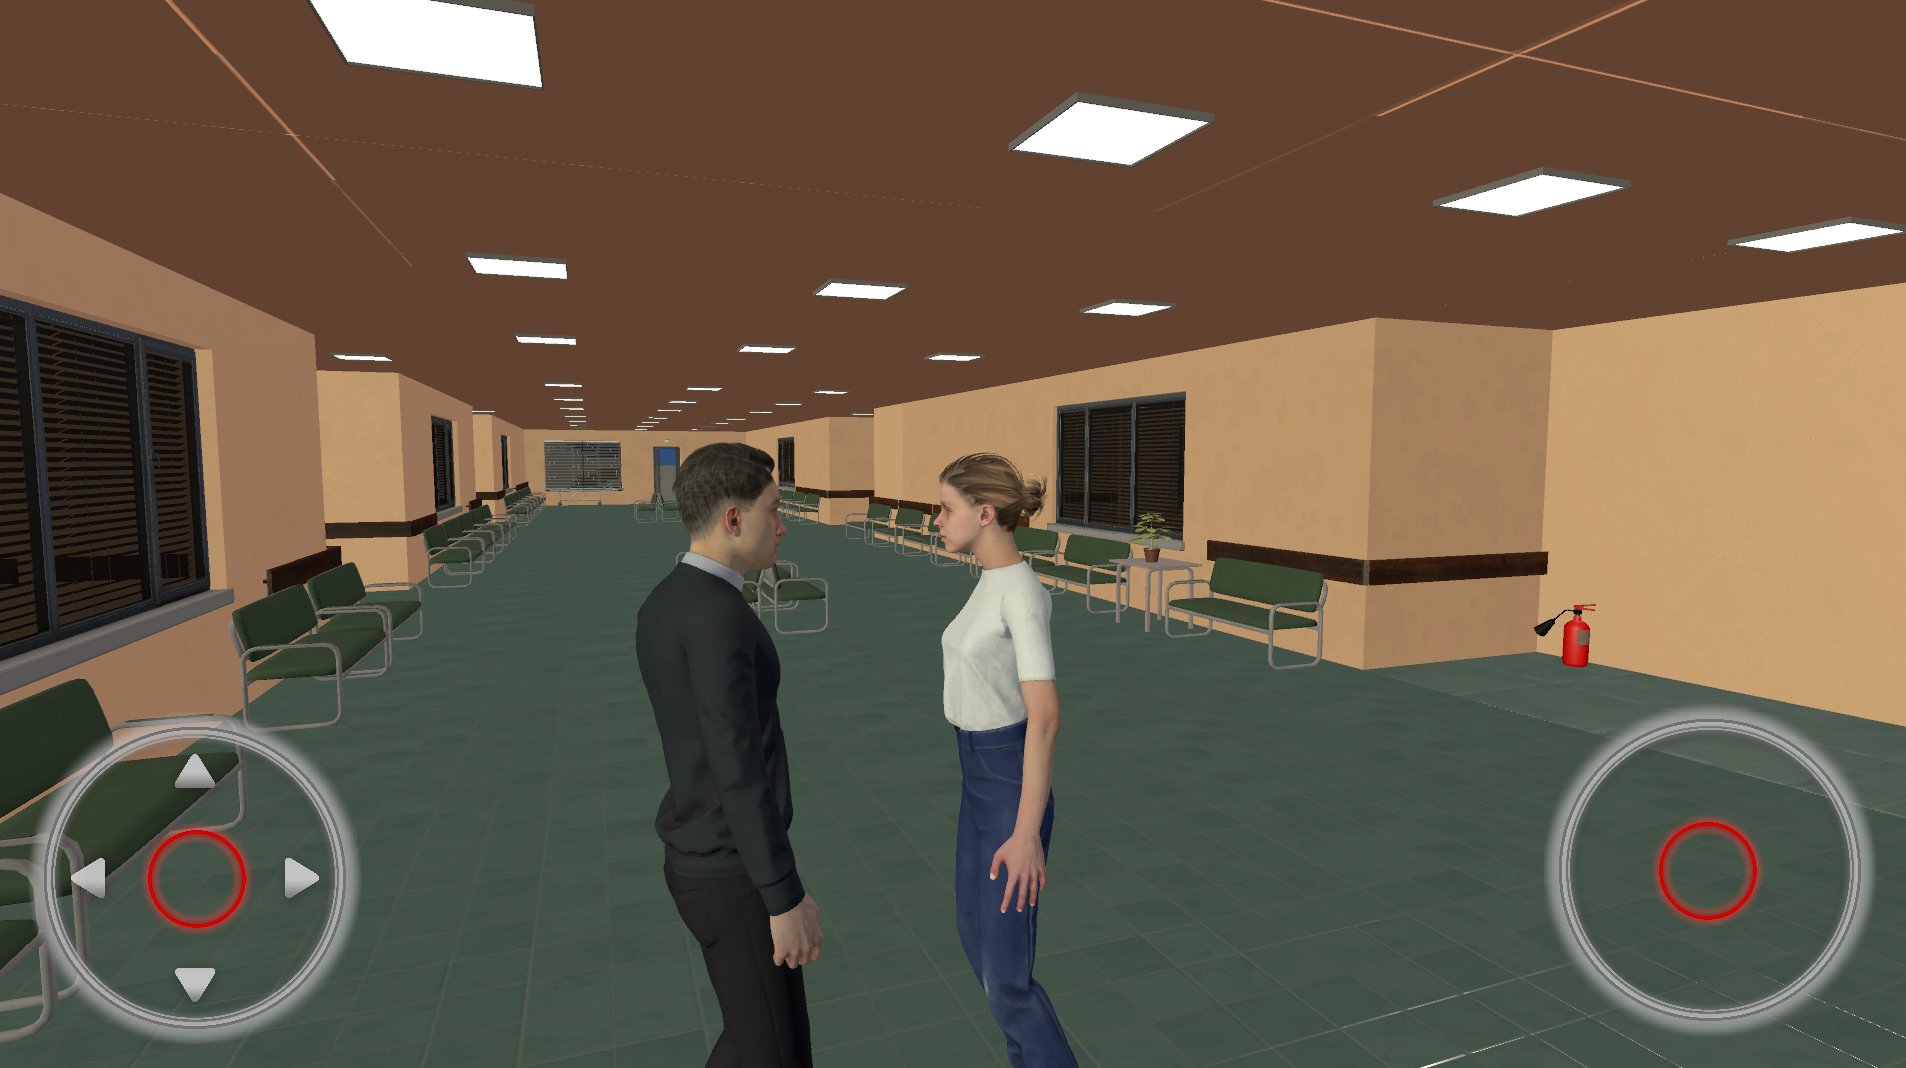
\includegraphics[width=0.5\textwidth, height=0.3\textheight]{Images/Waiting Area.png}
		\caption{Waiting Area}
\end{figure}
\\
\subsection{Patient Rooms:}	
Patient rooms are designed to offer a comfortable and healing atmosphere for patients during their hospital stay.
	\begin{figure}[h]
		\centering
		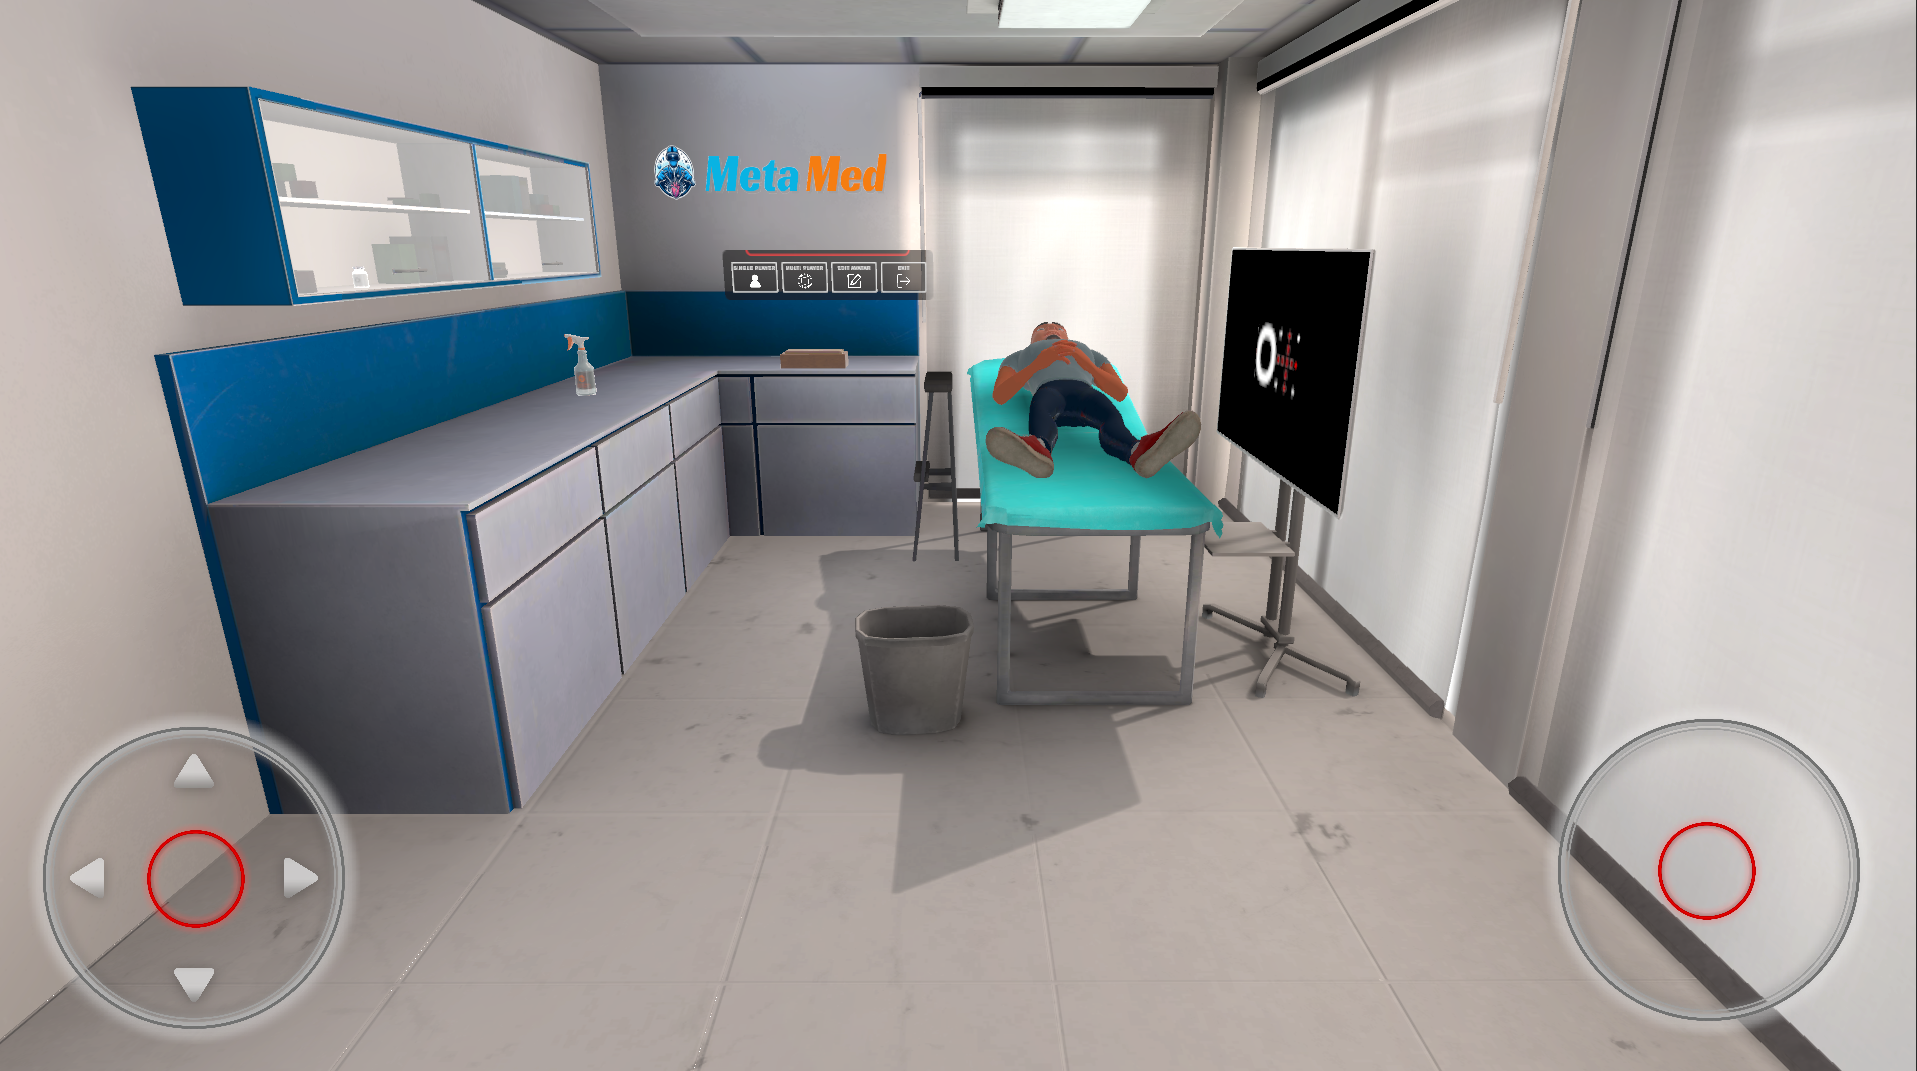
\includegraphics[width=0.5\textwidth, height=0.3\textheight]{Images/Patient Room.png}
		\caption{Patient Room}
		\label{fig:Patient-Room}
	\end{figure}	

\subsection{Patient Body:}	
Meta-verse Hospital has developed Patient Body to simulate patient interactions, offer realistic medical scenarios for training, and enhance healthcare professionals' virtual learning experiences.
\begin{figure}[h]
	\centering
	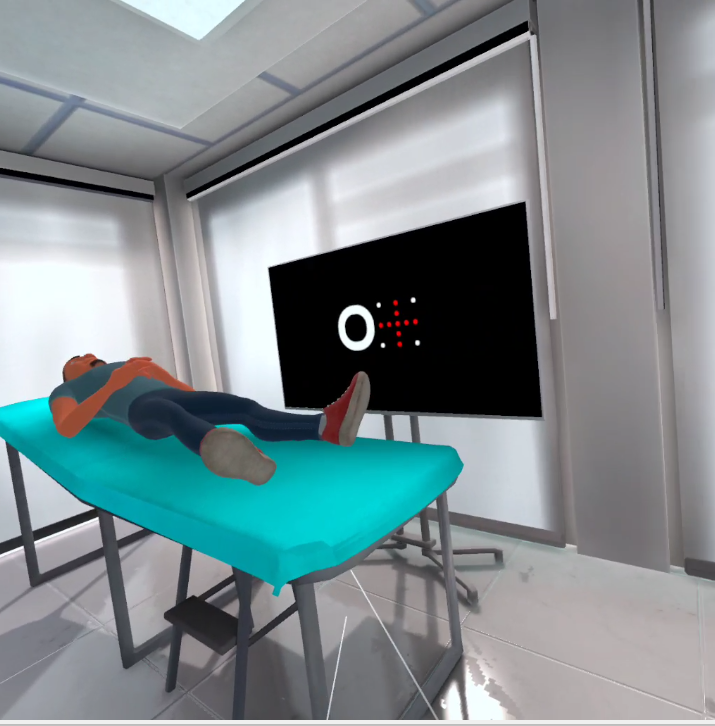
\includegraphics[width=0.5\textwidth, height=0.3\textheight]{Images/Patient Body.png}
	\caption{Patient Room}
	\label{fig:system-diagram}
\end{figure}	

	